\documentclass{article}

\usepackage{graphicx}
\usepackage{tikz}
\usepackage{tikzsymbols}
\usetikzlibrary{calc,patterns,shapes.geometric}
\pagestyle{empty}
\usepackage[margin=0pt]{geometry}
\geometry{papersize={14in,12in}}

\def\centerarc[#1](#2)(#3:#4:#5){\draw[#1] ($(#2)+({#5*cos(#3)},{#5*sin(#3)})$) arc (#3:#4:#5);}

\begin{document}
	\begin{figure}
		\centering
		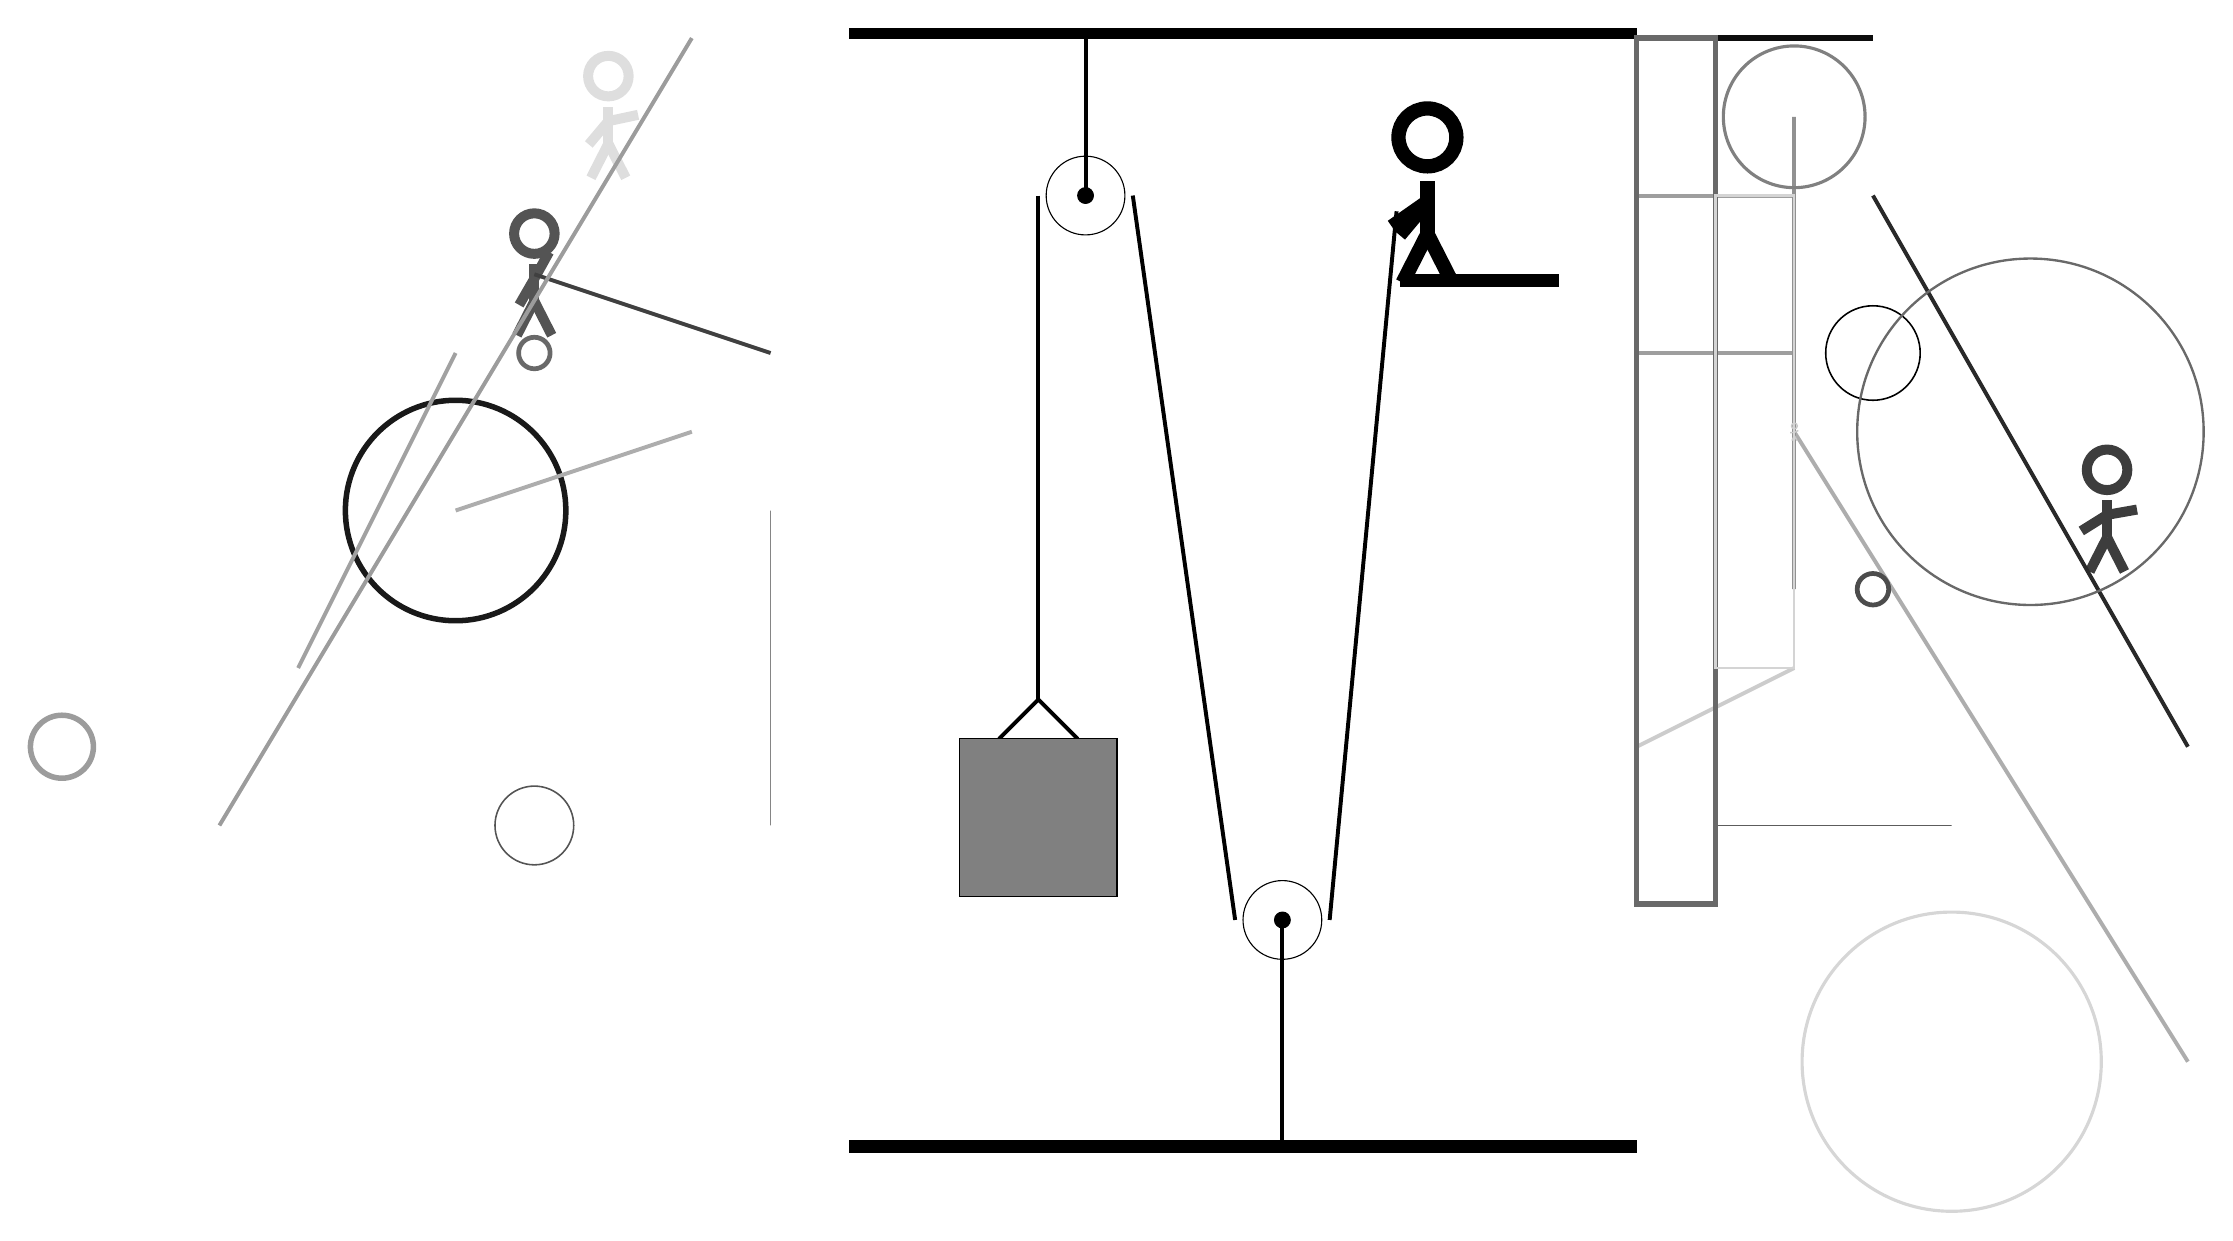
\begin{tikzpicture}
			%%%%% START %%%%%
			
			\draw[fill=black] (-2, 14) rectangle (8, 14.125);
			
			\draw[line width=0.7mm, color=black!84] (8, 14) rectangle (11, 14);
			
			\draw[line width=0.2mm, color=black!48] (-3, 4) rectangle (-3, 8);
			\node[line width=0.7mm, color=black!67] at (-6, 11) {\Strichmaxerl[7][60][61]};
			\node[line width=0.6mm, color=black!76] at (14, 8) {\Strichmaxerl[7][32][10]};
			\draw [line width=0.2mm, color=black!100](11, 10) circle (0.6);
			\draw[line width=0.5mm, color=black!38] (8, 10) rectangle (10, 12);
			\draw[line width=0.5mm, color=black!32](10, 9) -- (15, 1);
			
			\draw [line width=0.7mm, color=black!90](-7, 8) circle (1.4);
			\draw[line width=0.5mm, color=black!84](11, 12) -- (15, 5);
			\draw[line width=0.5mm, color=black!20](8, 5) -- (10, 6);
			
			\draw[line width=0.5mm, color=black!37](-7, 10) -- (-9, 6);
			
			\draw [line width=0.7mm, color=black!39](-12, 5) circle (0.4);
			\draw[line width=0.7mm, color=black!95] (8, 14) rectangle (11, 14);
			\node[line width=0.4mm, color=black!13] at (-5, 13) {\Strichmaxerl[7][50][12]};
			\draw[line width=0.5mm, color=black!43] (10, 13) rectangle (10, 7);
			\draw[line width=0.2mm, color=black!64] (9, 4) rectangle (12, 4);
			
			\draw[line width=0.5mm, color=black!75](-6, 11) -- (-3, 10);
			\draw [line width=0.4mm, color=black!16](12, 1) circle (1.9);
			\draw[line width=0.5mm, color=black!39](-4, 14) -- (-10, 4);
			\draw [line width=0.2mm, color=black!67](-6, 4) circle (0.5);
			\draw[line width=0.7mm, color=black!59] (9, 14) rectangle (8, 3);
			
			\draw [line width=0.4mm, color=black!50](10, 13) circle (0.9);
			
			\draw [line width=0.3mm, color=black!59](13, 9) circle (2.2);
			\draw[line width=0.5mm, color=black!32](-4, 9) -- (-7, 8);
			\node[line width=0.6mm, color=black!21] at (10, 9) {\Strichmaxerl[1][3][26]};
			\draw[line width=0.3mm, color=black!17] (10, 6) rectangle (9, 12);
			\draw [line width=0.6mm, color=black!59](-6, 10) circle (0.2);
			\draw [line width=0.6mm, color=black!70](11, 7) circle (0.2);
			
			
			\draw (3.5, 2.8) circle (0.5);
			\draw[fill=black] (3.5, 2.8) circle (0.1);
			\draw[line width=0.5mm] (3.5, 2.8) -- (3.5, 0);
			
			\draw (1, 12) circle (0.5);
			\draw[fill=black] (1, 12) circle (0.1);
			\draw[line width=0.5mm] (1, 14) -- (1, 12);
			
			\draw[line width=0.5mm](-0.1, 5.1) --  (0.4, 5.6) -- (0.9, 5.1);
			\draw[fill=black!50] (-0.6, 5.1) rectangle (1.4, 3.1);
			
			\draw[line width=0.5mm](0.4, 12) -- (0.4, 5.6);
			\centerarc[line width=0.5mm](1, 12)(180:0:0.6)
			\draw[line width=0.5mm](1.6, 12) -- (2.9, 2.8);
			\centerarc[line width=0.5mm](3.5, 2.8)(180:360:0.6)
			\draw[line width=0.5mm](4.1, 2.8) -- (4.95, 11.8);
			
			\node at (5.3, 12) {\Strichmaxerl[10][35][-130]};
			\draw[fill=black] (5, 11) rectangle (7, 10.85);
			
			\draw[fill=black] (-2, 0) rectangle (8, -0.15);
			
			%%%%% END %%%%%
		\end{tikzpicture}
	\end{figure}	
\end{document}